\section{EXCELLENCE}
\label{sec:excellence}

\subsection{Quality, innovative aspects and credibility of the research}
\label{sec:quality}

\subsubsection{Introduction}
\label{sec:introduction}

In Europe, prostate cancer is reported to be the most frequently diagnosed cancer of men and thus one of the leading cause of death of cancer~\footcite{Ferlay2013}. 
Currently, addressing this issue is a major public debate, in which the implementation of appropriate screening methods and subsequent treatments is key.

In this regard, the \ac{erspc} is conducted to investigate the potential benefits of a population-based screening~\footcite{Schroder2015}. 
The screening consists of a \ac{psa} test and depending of the \ac{psa} level measured, an additional ``blind'' biopsy is carried out. 
Despite the fact of a significant reduction of the prostate cancer mortality, the screening strategy employed suffers of a high rate of over-diagnosis and over-treatment~\cite{Delpierre2013,Schroder2015}, due to the fact that prostate cancer growth is characterized by two main types of evolution: slow and fast.
The slow-growing tumours account for up to~85~\% of all cancers and stay confined to the prostate gland, while the fast-growing tumours rapidly develop and metastasise to other organs, significantly affecting the morbidity and mortality rate.
Furthermore, prostate cancer is more likely to develop in specific regions of the prostate: around~70-80~\% of prostate cancers originate in the \ac{pz}, whereas~10-20~\% in the \ac{cg}, but appear to be more aggressive and more likely to invade other organs. 
\textbf{Thus, additionally to cancer detection, the screening methods need to provide an estimate of the cancer aggressiveness to allow clinicians to act accordingly.}

In addition, the investigators of the \ac{erspc} have come to the conclusion that the use of \emph{``multi-parametric \ac{mri} and the development of new markers are the hope for the future''}.
That is why, \ac{cad} systems revolved around mono- and multi-parametric \ac{mri} are currently developed by the medical imaging community, and were recently reviewed by Lema\^itre~\emph{et al.}~\footcite{Lemaitre2015}.
The \ac{cad} systems developed are designed under the same architecture as depicted in Fig.\,\ref{fig:wkfcad}. 
The available \ac{mri} modalities during prostate exam are \ac{t2w}-\ac{mri}, \ac{dw}-\ac{mri}, \ac{dce}-\ac{mri}, and \ac{mrsi}. 
Additionally, \ac{adc} map is based on the computation of a coefficient derived from multiple \ac{dw}-\ac{mri}.
\textbf{Currently, no \ac{cad} system has been developed using all the available modalities and thus discarding their potential discriminating power to diagnose prostate cancer.}
\begin{figure*}[h]
  \centering

  % Define block styles used later

  \tikzstyle{module}=[draw, draw=blue!80, text width=10em, 
  text centered, minimum height=5em, minimum width = 15em, drop shadow, rounded corners,
  fill=blue!30]
  
  \tikzstyle{vecArrow} = [thick, decoration={markings,mark=at position
    1 with {\arrow[semithick]{open triangle 60}}},
  double distance=1.4pt, shorten >= 5.5pt,
  preaction = {decorate},
  postaction = {draw,line width=1.4pt, white,shorten >= 4.5pt}]

  % Define distances for bordering
  \def\blockdist{1.5}
  \def\edgedist{2.5}

  \begin{tikzpicture}[node distance=3cm,thick,scale=0.4, every node/.style={scale=0.4},path image/.style={
      path picture={
        \node at (path picture bounding box.center) {
          \includegraphics[width=1cm]{#1}
        };}}]
    \tikzstyle{conefill} = [path image=,fill opacity=0.8]
    \node[module=above:pre] (pre) at (4.5,-2.6) {\Large Pre-processing};
    \node[module,below of=pre] (seg) {\Large Segmentation};
    \node[module,below of=seg] (reg) {\Large Registration};

    \path[->,dashed] (seg.west) edge [bend right=70] node {} (reg.west);
    \path[->,dashed] (reg.east) edge [bend right=70] node {} (seg.east);

    \draw[->] (pre)--(seg);
    \draw[->] (seg)--(reg);

    \begin{pgfonlayer}{background}
      \path (pre.west |- pre.north)+(-0.9,1.0+\blockdist) node (a) {};
      \path (reg.east |- reg.south)+(+0.9,-0.5) node (b) {};
      
      \path[fill=blue!10,rounded corners, draw=blue!20, dashed] (a) rectangle (b);
    \end{pgfonlayer}
    
    \path (pre.north) +(0,+\blockdist) node (bgreg) {\Large Image regularization};

    \begin{scope}[node distance=10cm]
      \node[module] (det) [below right=0cm and 3cm of pre] {\Large Features detection};
    \end{scope}
    \begin{scope}[node distance=3.5cm]
      \node[module,above of=det] (roi) {\Large ROIs\\detection/selection};
    \end{scope}
    \node[module,below of=det] (sel) {\Large Features\\selection/extraction};
    \node[module,below of=sel] (cla) {\Large Features\\classification/fusion};

    \draw[->] (roi)--(det);
    \draw[->] (det)--(sel);
    \draw[->] (sel)--(cla);

    \begin{pgfonlayer}{background}
      \path (roi.west |- roi.north)+(-0.25,0.8) node (c) {};
      \path (roi.east |- roi.south)+(+0.25,-0.25) node (d) {};
      
      \path[fill=blue!20,rounded corners, draw=blue!25, dashed] (c) rectangle (d);
    \end{pgfonlayer}

    \path (roi.west |- roi.north) +(.6,0.4) node (bgfea) {\Large \textbf{CADe}};

    \begin{pgfonlayer}{background}
      \path (det.west |- det.north)+(-0.25,0.8) node (c) {};
      \path (cla.east |- cla.south)+(+0.25,-0.25) node (d) {};
      
      \path[fill=blue!20,rounded corners, draw=blue!25, dashed] (c) rectangle (d);
    \end{pgfonlayer}

    \path (roi.west |- det.north) +(.6,0.4) node (bgfea) {\Large \textbf{CADx}};     

    % Define the place where the arrow should start anf finish
    \path (seg.east |- seg.north)+(+0.9,0) node (e) {};
    \path (sel.west |- seg.north)+(-0.8,0) node (f) {};

    \draw[double distance =3pt,preaction={-triangle 90,thin,draw,shorten >=-1mm}] (e) -- (f) node[midway,above] {\Large Regularized data};

    \begin{scope}[yshift=34,xshift=-86]
      \transparent{0.6}\draw[path image=content/proposal/figures/tikzimage/t2.eps] (0,0) rectangle (1.0,1.0);
    \end{scope}

    \begin{scope}[yshift=31,xshift=-83]
      \transparent{0.6}\draw[path image=content/proposal/figures/tikzimage/t2.eps] (0,0) rectangle (1.0,1.0);
    \end{scope}

    \begin{scope}[yshift=28,xshift=-80]
      \transparent{0.8}\draw[path image=content/proposal/figures/tikzimage/t2.eps] (0,0) rectangle (1.0,1.0);
      \path (0,0)+(-1.5,0.3) node {\Large T$_2$-W MRI};
    \end{scope}

    \begin{scope}[yshift=-33,xshift=-86]
      \transparent{0.6}\draw[path image=content/proposal/figures/tikzimage/t2.eps] (0,0) rectangle (1.0,1.0);
    \end{scope}

    \begin{scope}[yshift=-36,xshift=-83]
      \transparent{0.6}\draw[path image=content/proposal/figures/tikzimage/t2.eps] (0,0) rectangle (1.0,1.0);
    \end{scope}

    \begin{scope}[yshift=-39,xshift=-80]
      \transparent{0.8}\draw[path image=content/proposal/figures/tikzimage/t2.eps] (0,0) rectangle (1.0,1.0);
      \path (0,0)+(-1.2,0.3) node {\Large T$_2$ map};
    \end{scope}

    \begin{scope}[yshift=-100,xshift=-86]
      \transparent{0.6}\draw[path image=content/proposal/figures/tikzimage/dce.eps] (0,0) rectangle (1.0,1.0);
    \end{scope}

    \begin{scope}[yshift=-103,xshift=-83]
      \transparent{0.6}\draw[path image=content/proposal/figures/tikzimage/dce.eps] (0,0) rectangle (1.0,1.0);
    \end{scope}

    \begin{scope}[yshift=-106,xshift=-80]
      \transparent{0.8}\draw[path image=content/proposal/figures/tikzimage/dce.eps] (0,0) rectangle (1.0,1.0);
      \path (0,0)+(-1.5,0.3) node {\Large DCE MRI};
    \end{scope}

    \begin{scope}[yshift=-167,xshift=-86]
      \transparent{0.6}\draw[path image=content/proposal/figures/tikzimage/dwi1.eps] (0,0) rectangle (1.0,1.0);
    \end{scope}

    \begin{scope}[yshift=-170,xshift=-83]
      \transparent{0.6}\draw[path image=content/proposal/figures/tikzimage/dwi1.eps] (0,0) rectangle (1.0,1.0);
    \end{scope}

    \begin{scope}[yshift=-173,xshift=-80]
      \transparent{0.8}\draw[path image=content/proposal/figures/tikzimage/dwi1.eps] (0,0) rectangle (1.0,1.0);
      \path (0,0)+(-1.5,0.3) node {\Large DW MRI};
    \end{scope}

    \begin{scope}[yshift=-234,xshift=-86]
      \transparent{0.6}\draw[path image=content/proposal/figures/tikzimage/adc.eps] (0,0) rectangle (1.0,1.0);
    \end{scope}

    \begin{scope}[yshift=-237,xshift=-83]
      \transparent{0.6}\draw[path image=content/proposal/figures/tikzimage/adc.eps] (0,0) rectangle (1.0,1.0);
    \end{scope}

    \begin{scope}[yshift=-240,xshift=-80]
      \transparent{0.8}\draw[path image=content/proposal/figures/tikzimage/adc.eps] (0,0) rectangle (1.0,1.0);
      \path (0,0)+(-1.5,0.3) node {\Large ADC};
    \end{scope}

    \begin{scope}[yshift=-301,xshift=-86]
      \transparent{0.6}\draw[path image=content/proposal/figures/tikzimage/mrsi.eps] (0,0) rectangle (1.0,1.0);
    \end{scope}

    \begin{scope}[yshift=-304,xshift=-83]
      \transparent{0.6}\draw[path image=content/proposal/figures/tikzimage/mrsi.eps] (0,0) rectangle (1.0,1.0);
    \end{scope}

    \begin{scope}[yshift=-307,xshift=-80]
      \transparent{0.8}\draw[path image=content/proposal/figures/tikzimage/mrsi.eps] (0,0) rectangle (1.0,1.0);
      \path (0,0)+(-1,0.3) node {\Large MRSI};
    \end{scope}

    \path (pre.west |- roi.north)+(-3.5,1.0+\blockdist) node (g) {};
    \path (reg.west |- cla.south)+(-3.5,-0.5) node (h) {};

    \draw[decorate,decoration={brace,raise=6pt,amplitude=10pt}, thick]
    (g)--(h) ;
    
    \path (seg.west |- seg.north)+(-2.5,0) node (i) {};
    \path (seg.west |- seg.north)+(-0.9,0) node (j) {};
    
    \draw[double distance =3pt,preaction={-triangle 90,thin,draw,shorten >=-1mm}] (i) -- (j);   

    \path (sel.east |- seg.north)+(2,0) node (k) {};
    \path (sel.east |- seg.north)+(0.5,0) node (l) {};
    
  \end{tikzpicture}
  \caption{Common \ac{cad} framework based on \ac{mri} images used to detect prostate cancer.}
  \label{fig:wkfcad}
\end{figure*}

% \begin{figure*}
%   \centering
%   \hspace*{\fill}
%   \subfigure[\ac{t2w}-\ac{mri} slice of an healthy prostate acquire with a 1.5 Tesla \ac{mri}. The blue contour represents the \ac{cg} while the \ac{pz} corresponds to the green contour.]{\label{subfig:t2whealthy}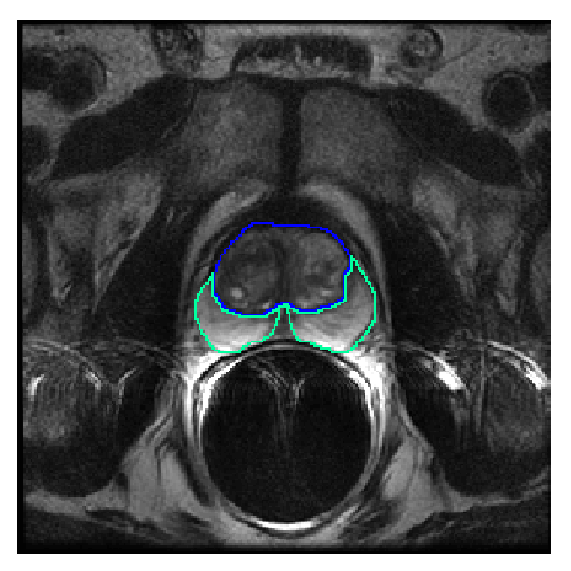
\includegraphics[width=0.3\linewidth]{12_figures/figures/t2w/t2w_healthy.eps}} \hfill
%   \subfigure[\ac{t2w}-\ac{mri} slice of a prostate with a \ac{cap} highlighted in the \ac{pz} using a 3.0 Tesla \ac{mri} scanner.]{\label{subfig:t2wcancerpz}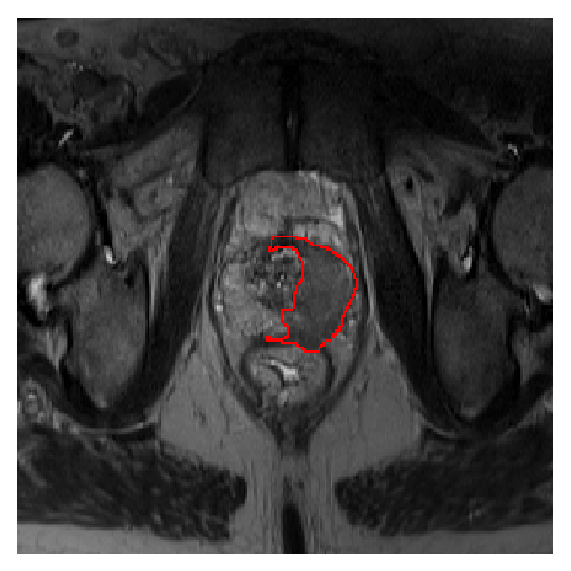
\includegraphics[width=0.3\linewidth]{12_figures/figures/t2w/t2w_cancer_pz.eps}} \hfill
%   \subfigure[\ac{t2w}-\ac{mri} slice of a prostate with a \ac{cap} highlighted in the \ac{cg} using a 3.0 Tesla \ac{mri} scanner.]{\label{subfig:t2wcancercg}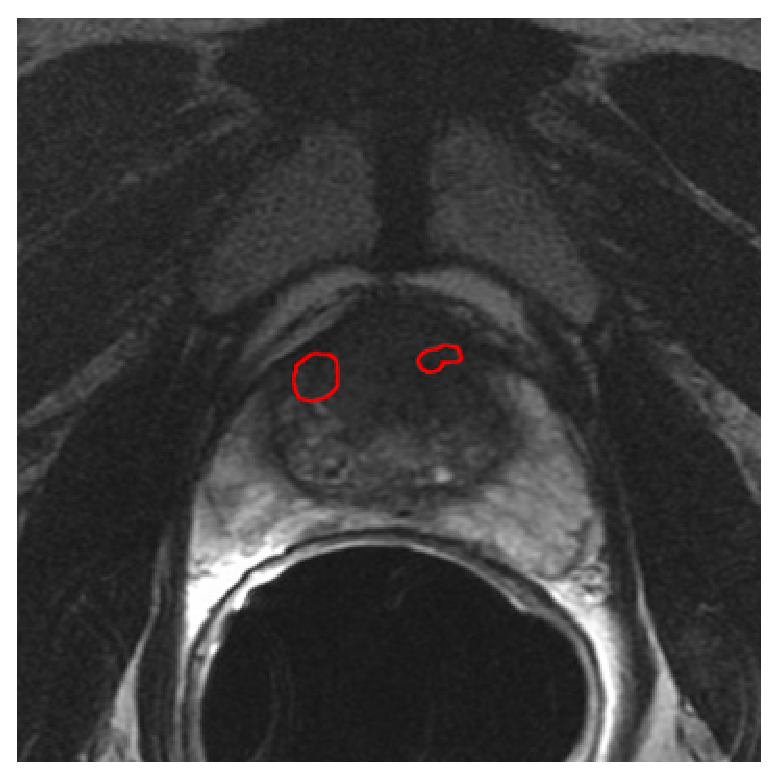
\includegraphics[width=0.3\linewidth]{12_figures/figures/t2w/t2w_cancer_cg.eps}}
%   \hspace*{\fill}
%   \caption{Rendering of \ac{t2w}-\ac{mri} prostate image with both 1.5 and 3.0 Tesla \ac{mri} scanner.}
%   \label{fig:t2w}
% \end{figure*}

% \begin{figure*}
%   \centering
%   \hspace*{\fill}
%   \subfigure[]{\label{subfig:t1w}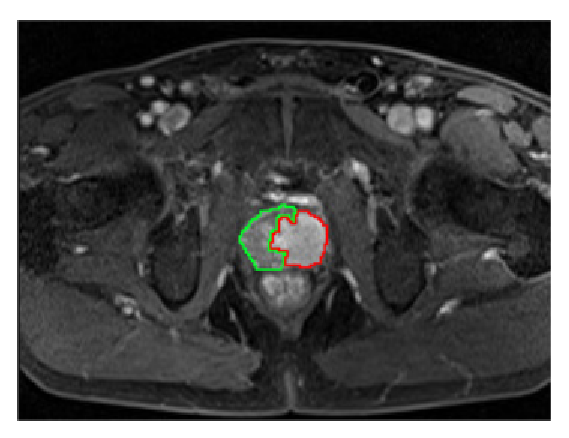
\includegraphics[width=0.35\linewidth]{12_figures/figures/dce/slice.eps}} \hfill
%   \subfigure[]{\label{subfig:dce}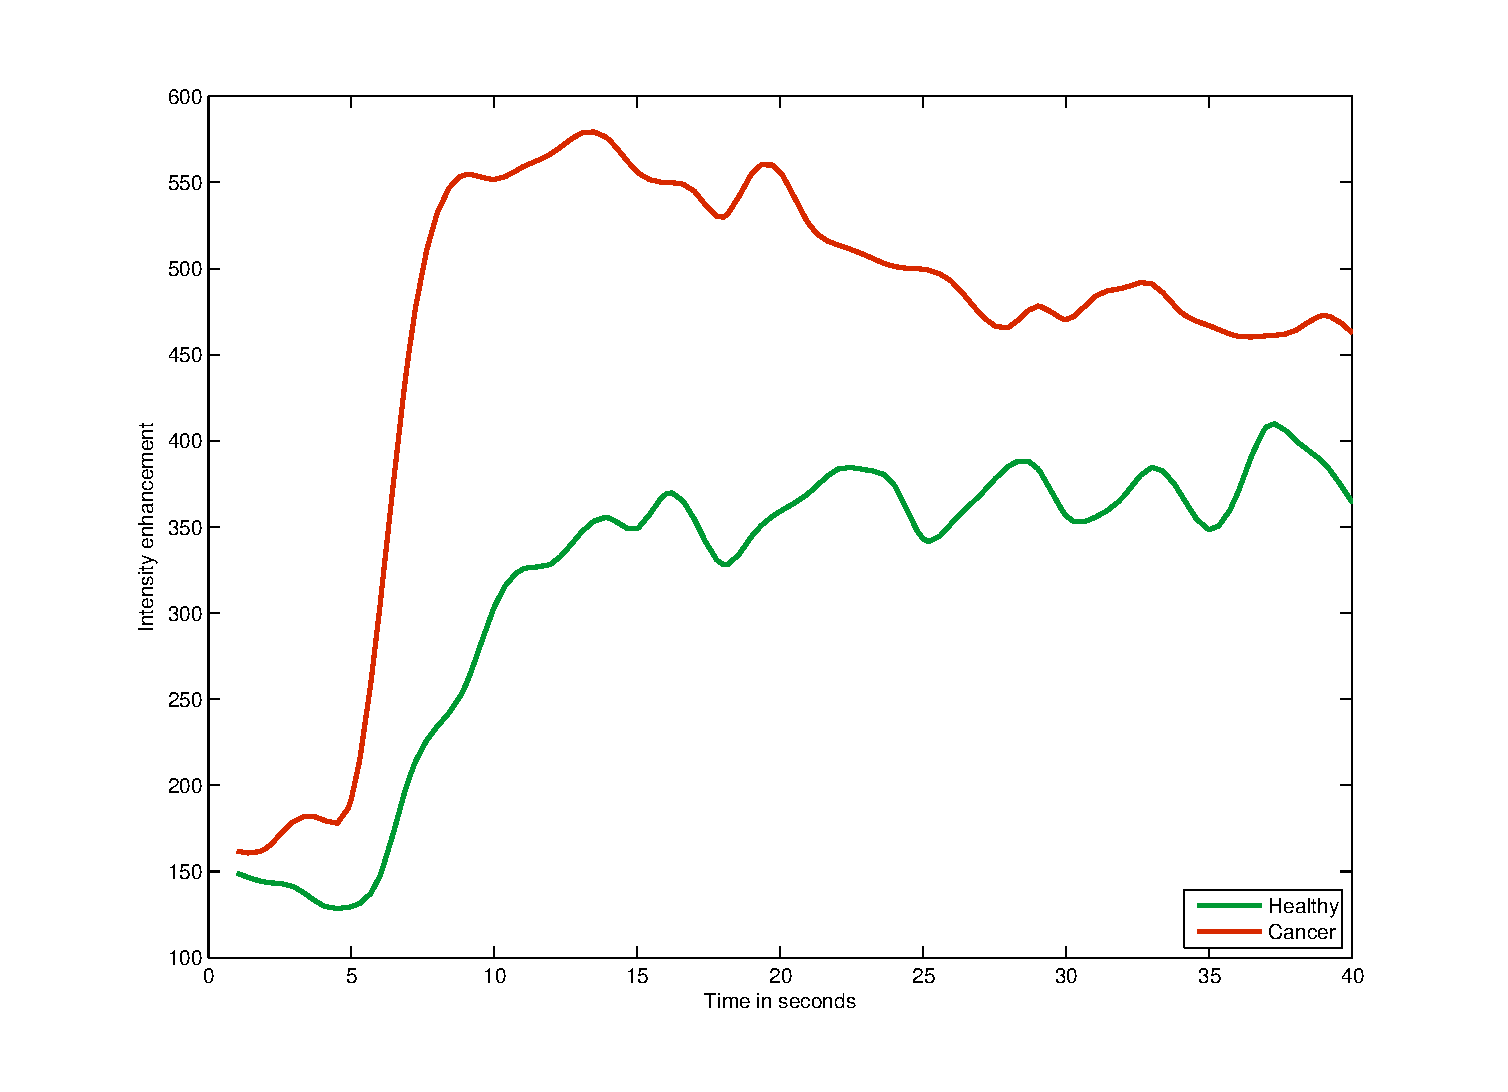
\includegraphics[width=0.35\linewidth]{12_figures/figures/dce/dce_cancer_healthy.eps}}
%   \hspace*{\fill}
%   \caption{Illustration of: \subref{subfig:t1w} \ac{t1w}-\ac{mri} image and \subref{subfig:dce} typical enhancement signals observed in \ac{dce}-\ac{mri} analysis collected with a 3.0 Tesla \ac{mri} scanner. The red curve is typical from \ac{cap} while the green curve is characteristic of healthy tissue.}
%   \label{fig:dceana}
% \end{figure*}

% \begin{figure}
%   \centering
%   \hspace*{\fill}
%   \subfigure[]{\label{subfig:dwi}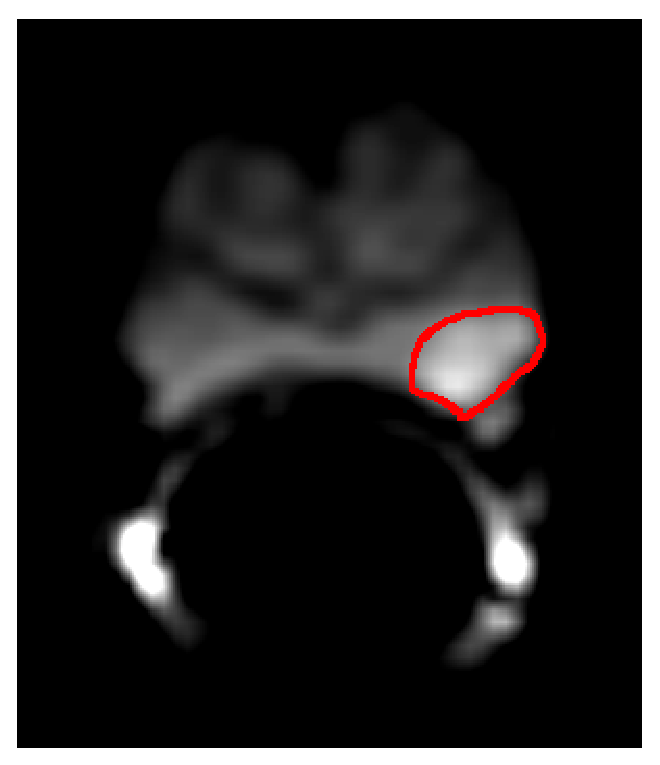
\includegraphics[height=0.15\textheight]{12_figures/figures/dwi/dwi_cancer.eps}} \hfill
%   \subfigure[]{\label{subfig:adc}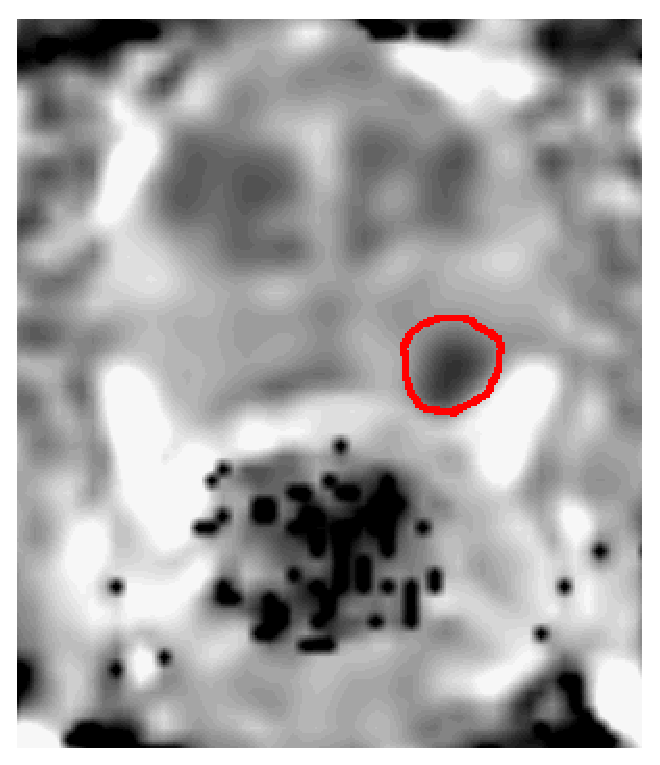
\includegraphics[height=0.15\textheight]{12_figures/figures/dwi/adc_cancer.eps}}
%   \hspace*{\fill}
%   \caption{Illustration of: \subref{subfig:dwi} \ac{dw}-\ac{mri} and \subref{subfig:adc} \ac{adc} map. The signal intensity corresponding to cancer are inversely correlated on these two types of imaging techniques. The cancer is highlighted in red.}
%   \label{fig:dwi}
% \end{figure}

% \begin{figure*}
%   \centering
%   \hspace*{\fill}
%   \subfigure[]{\label{subfig:mrsihea}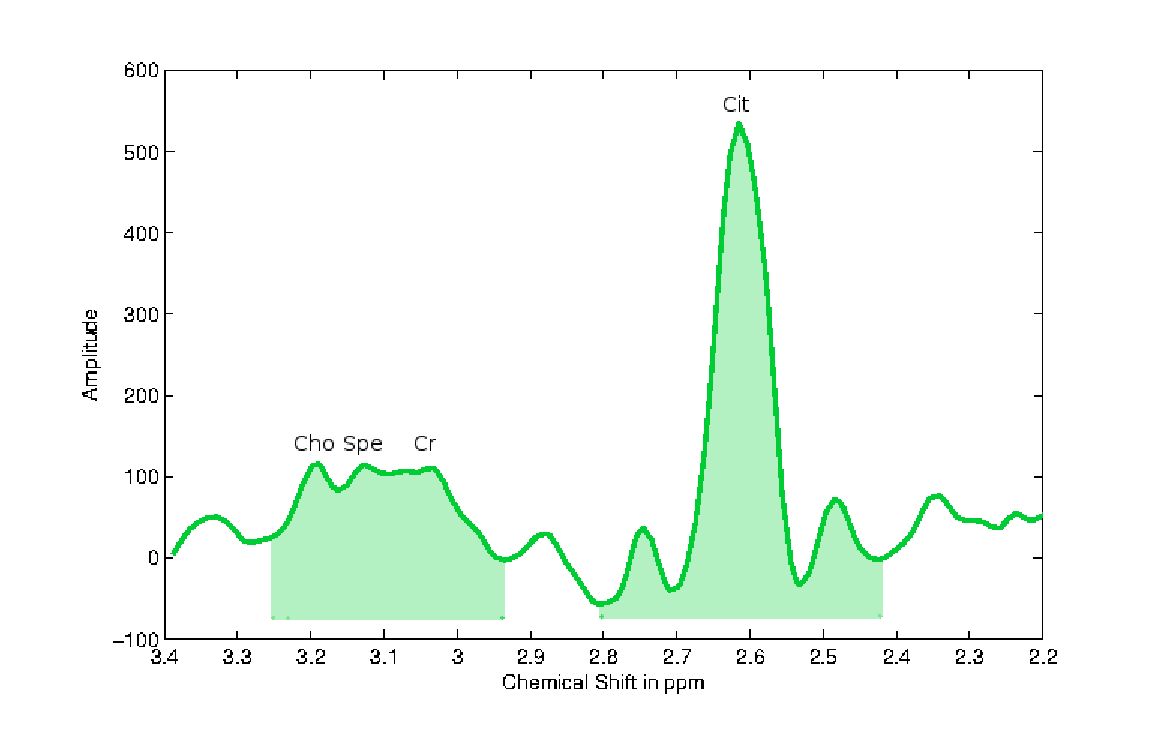
\includegraphics[width=0.45\linewidth]{12_figures/figures/mrsi/mrsi_healthy.eps}} \hfill
%   \subfigure[]{\label{subfig:mrsican}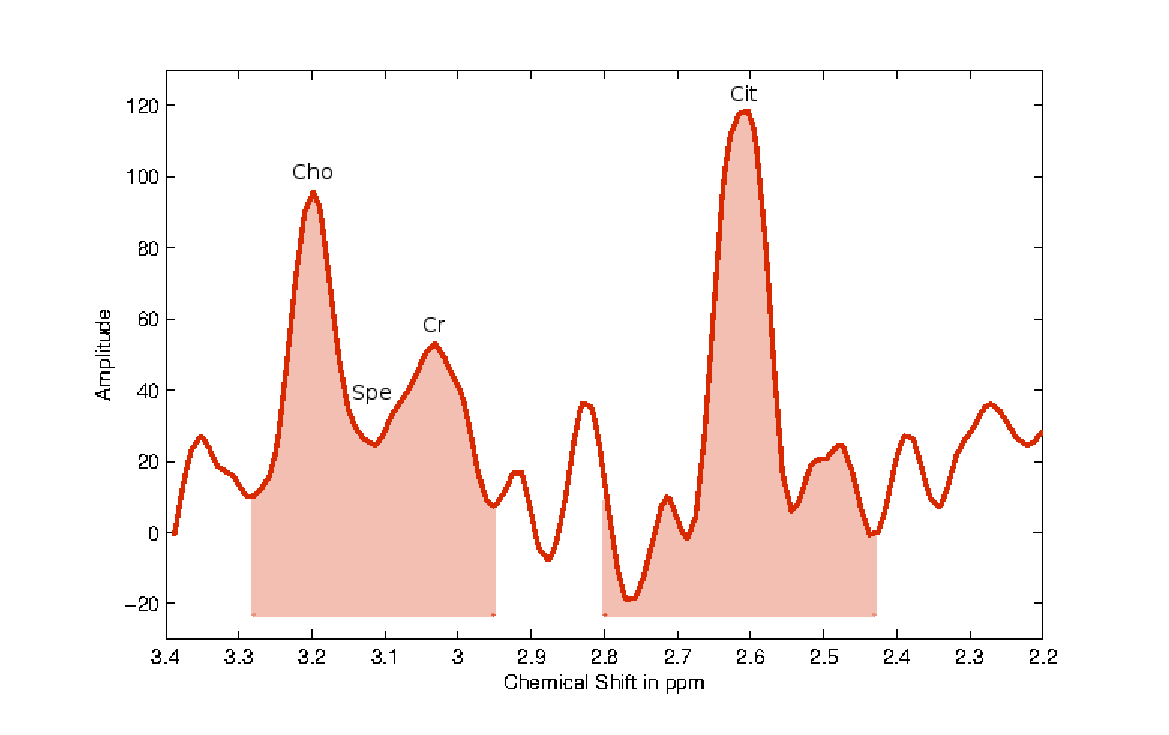
\includegraphics[width=0.45\linewidth]{12_figures/figures/mrsi/mrsi_cancer.eps}}
%   \hspace*{\fill}
%   \caption{Illustration of an \ac{mrsi} spectrum both \subref{subfig:mrsihea} healthy and \subref{subfig:mrsican} cancerous voxel with a 3.0 Tesla \ac{mri}. The highlighted areas corresponds to the related concentration of the metabolites which is computed by integrating the area under each peak. Acronyms: Choline (Cho), Spermine (Spe), Creatine (Cr) and Citrate (Cit).}
%   \label{fig:mrsi}
% \end{figure*}

%%% Local Variables: 
%%% mode: latex
%%% TeX-master: "../../../main"
%%% End: 

The closest attempts used three of these modalities (i.e., \ac{t2w}-\ac{mri}, \ac{dw}-\ac{mri}, \ac{dce}-\ac{mri}) and discarded \ac{mrsi}~\footcite{Litjens2014}\textsuperscript{,}\footcite{Viswanath2011}.
This latter, however, has been shown to be extremely helpful to grade cancer aggressiveness particularly in the \ac{cg}~\footcite{Vos2015}, which is the most challenging zone in terms of cancer detection.
\textbf{Furthermore, the current researches solely focus on the delineation of prostate cancers rather than on the cancer aggressiveness assessment.}

Therefore, the aim of this project is to design a \ac{cad} system able to both detect and assess prostate cancers using all currently available multi-parametric \ac{mri} modalities.
{\color{red} drastically improve here}
The architecture of our \ac{cad} system will imply the following investigations: 
\begin{enumerate}
\item Pre-processing to enhance the quality of \ac{mri} images (bias field correction, denoising, and normalisation),
\item Segmentation of prostate zones using multi-parametric \ac{mri} and deep-learning,
\item Registration of multi-parametric \ac{mri} using spline-based non-linear differmorphism,
\item Detection and assessment of prostate cancers using using multi-parametric \ac{mri} and deep-learning,
\item Identification of markers by inspection of the neural-network and transfer to classical machine learning approach.
\item Grading using standard PI-RADS
\end{enumerate}
These methodologies will be extensively presented and argued in Sect.\,\ref{sec:methodologies}.

\subsubsection{Research methodologies}
\label{sec:methodologies}

\paragraph{Data acquisition}

\paragraph{Pre-processing}

\Ac{mri} images are corrupted by different phenomena: (i) bias field, (ii) noise, and (iii) inter-patient variations.
In this regard, particular attention to correct each of these drawbacks will be addressed.

\Ac{mri} images are affected by the inhomogeneity of the \ac{mri} field called bias field, resulting in a smooth variation of the intensities.
Although bias correction methods are commonly used to enhance brain \ac{mri} images~\footcite{Vovk2007}, only one \ac{cad} system for prostate has reported to use such pre-processing~\footcite{Viswanath2009}.
The same authors performed an empirical evaluation of the state-of-the-art methods~\footcite{viswanath2011empirical} concluding that N3 algorithm~\footcite{Sled1998} yields to better classification results than other methods~\footcite{Styner2000}\textsuperscript{,}\footcite{Cohen2000}.
Recently, Lin~\emph{et al.}~\footcite{Lin2011} proposed a method combining the N3 algorithm with the FCM algorithm~\footcite{Ahmed2002} which outperforms the original methods in terms of breast segmentation.
\textbf{Therefore, we will perform an empirical comparison of these state-of-the-art methods~\footcite{Sled1998}\textsuperscript{,}\footcite{Styner2000}\textsuperscript{,}\footcite{Cohen2000}\textsuperscript{,}\footcite{Lin2011}, by ensuring the benefits of the method of Lin~\emph{et al.} for our specific application.}

Apart of the bias field, \Ac{mri} images are also degraded due to a Rician noise. Similarly to bias correction, only two \ac{cad} systems for prostate denoised images using wavelet-based techniques~\footcite{Mallat2008}\textsuperscript{,}\footcite{Pizurica2003}, offering a proper theoretical baseline for Rician corruption~\footcite{Nowak1999}.
Non-Local Means-based denoising techniques have never been used for \ac{mri} prostate images, but extensively and successfully for other \ac{mri} applications~\footcite{Manjon2008}.
\textbf{Thus, we will perform an empirical evaluation of the Non-Local Means-based techniques~\footcite{Manjon2012}\textsuperscript{,}\footcite{Coupe2011} and wavelet-based technique\footcite{Pizurica2003} to select the appropriate method to our application.}

\ac{cad} systems are based on machine learning classifiers which are trained to differentiate cancerous from healthy tissue.
The classification performance of these classifiers highly relies on the consistency of the dataset.
Subsequently, one can emphasize the desire to reduce the inter-patient variability of the \ac{mri} dataset.
In this regard, each patient dataset needs to be standardised/normalised to common basis, modality by modality.
Only two methods have been used in \ac{cad} for prostate: the first method consists in normalising the images via the $z$-score, while the second technique is based on a linear normalisation by parts~\footcite{Madabhushi2006a}.
Lema\^itre~\emph{et al.}~\footnote{This work is submitted for publication.} developed a normalisation technique using the Rician properties of the \ac{mri} signal, which outperforms the previous methods for \ac{t2w}-\ac{mri} images.
\textbf{Thus, we will extend this work to the other modalities \ac{dce}-\ac{mri} and \ac{dw}-\ac{mri}}.

\ac{mrsi} is a modality related to one dimensional signal, thus enhancing techniques differs from the one used in \ac{mri}.
The \ac{mrsi} spectra have to be corrected for several phenomena: phase correction, water and lipid residuals filtering, baseline correction, frequency alignment, and normalisation.
This set of enhancement techniques already have been investigated by Lema\^itre~\emph{et al.}~\footcite{Lemaitre2011}, in a study focusing solely on the \ac{mrsi} modality for prostate cancer detection; \textbf{this knowledge will be the basis of \ac{mrsi} enhancement.}

\paragraph{Segmentation}

To achieve robust cancer detection, the classification has to be carried out only on the prostate area, motivating the need to perform a segmentation of the organ in the \ac{mri} images.
Furthermore, as mentioned in Sect.\,\ref{sec:introduction}), the membership \emph{a priori} of a voxel to a specific prostate zone has a high potential to increase the performance to evaluate the aggressiveness of prostate cancer.
Therefore, the prostate zones need to be segmented instead of solely the prostate organ.
In this regard, only the work of Litjens~\emph{et al.} performed a zonal segmentation of the prostate using probabilistic multi-atlas approach~\footcite{Litjens2014}.
However, the segmentation was performed only considering the \ac{t2w}-\ac{mri} modality and the \ac{adc} map.
Moreover, although atlas-based methods are robust to intensity variations, they lack of accuracy in the boundary delineations~\footcite{Ghose2012}.
The potential of machine learning methods to carry out such task is currently underestimated, but has been shown to be suitable in combination with the other approach~\footcite{ghose2012graph}.
\textbf{Thus, we will design a hybrid system based on \ac{cnn} and \ac{asm} using all multi-parametric images to perform zonal segmentation.}
The choice of \ac{cnn} is motivated by the recent breakthrough of deep-learning in multiple fields of computer vision.
Deep-learning, however, has still not be extensively used in the field of medical imaging as attested by the organisation of the first workshop specifically dedicated to this topic at MICCAI 2015. 
Deep-learning relies on a data-driven training stage in which large amount of data are required, which is a serious drawback in medical imaging.
However, this is the problematic tackled by the field of transfer learning which will allow to deploy deep-learning to medical imaging.

\paragraph{Registration}

In multi-parametric \ac{mri}, the data are collected in a sequential manner, involving a possible misalignment between the different modalities.
Mitra~\emph{et al.}~\footcite{Mitra2012a} developed an automatic multi-modal non-rigid registration method, which has been shown to outperform the state-of-the-art methods.
This method was initially used for registration between \ac{t2w}-\ac{mri} and \ac{us} prostate images, \textbf{therefore, we will extend this method to align our multi-parametric \ac{mri} dataset.}

\paragraph{Detection and assessment}

Up to know, the \ac{cad} systems developed solely focus on the detection of prostate cancers, omitting a real-assessment of the potential lesions detected.
The detection of cancers is commonly performed using machine leaning classifiers, designing frameworks as depicted in Fig.\,\ref{fig:wkfcad}.
These frameworks rely on two compulsory stages and an intermediate optional one: (i) features detection, (ii) features selection/extraction and (iii) features classification.
Lema\^itre~\emph{et al.} extensively reviewed researches carried out in each of this stage for the development of \ac{cad} for prostate cancer~\footcite{Lemaitre2015}.
These stages are organised in a sequential manner and thus stages upstream part of the features classification will have a tremendous importance on the classification performance.
Consequently, the use of discriminative features is certainly key and most probably the bottleneck of \ac{cad} systems, justifying the attention given by researchers to evaluate multitude of low- and high-level visual features, inspired by computer vision or biology.
As aforementioned, deep-learning has been recently shown to one of the most successful machine learning technique for broad types of classification tasks.
\ac{cnn} has the ability to generate automatically low- and high-level visual features in the network itself~\footcite{Zeiler2013} by only supplying the raw data as inputs.
Furthermore, \ac{cnn} can be trained using the Gleason grade obtained through biopsy in order to get an assessment of the aggressiveness of the cancer.
\textbf{Thus, we will use \ac{cnn} to perform the detection and the assessment of prostate cancer. In addition, we will investigate the low- and high-level features to potentially find new bio-markers which can be used by clinicians or other machine learning methods.}

\paragraph{Evaluation using \acs*{pirads}}

The \ac{esur} together with the \ac{acr} recently published the \ac{pirads}, which is a standard way to assess and report prostate lesions using multi-parametric \ac{mri}.
This standard allows to report a score depending of multiple criteria such as signal intensity, texture, size of lesion, modality, prostate zones, etc.
None of the current \ac{cad} systems offer a \ac{pirads} score when detecting potential lesions in multi-parametric \ac{mri}.
\textbf{Thus, we will report the output of our classification framework in terms of \ac{pirads} score, applying the provided criterion.}

\subsection{Clarity and quality of transfer of knowledge/training for the development of the researcher in light of the research objectives}
\label{sec:transfer}


\subsection{Quality of the supervision and the hosting arrangements}
\label{sec:supervision}

\subsubsection*{Qualifications and experience of the supervisor(s)}


\paragraph{Career development}

\subsection{Capacity of the researcher to reach and re-enforce a position of professional maturity in research}
\label{sec:maturity}
